\documentclass[a4paper,english,twoside,10pt]{article}

\usepackage[left=2.5cm,right=2.5cm,bottom=3cm]{geometry}
\usepackage{babel}
\usepackage{amsmath}
\usepackage{enumitem}
% \usepackage{listings}
\usepackage{caption}
\usepackage{csquotes} % Auto open/close quote mark
\MakeOuterQuote{"} % Use quote mark as container for smart quotation system
\usepackage[stretch=10]{microtype} % Better impagination due to micro font shrinking and stretching
\usepackage[justification=centering]{caption}
\usepackage{tikz}
% \usetikzlibrary{arrows,shapes,calc,babel,positioning,fit}
\usepackage[breaklinks]{hyperref}
\usepackage{minted}
\usemintedstyle{perldoc}
\usepackage[acronym]{glossaries}
\usepackage{authoraftertitle} % Get title and author available as commands

\newcommand{\listingautorefname}{Listing}
\newcommand{\mclr}{\(\overline{\mbox{MCLR}}\)\ }
\newcommand{\vdd}{V\textsubscript{DD}}

% \tikzstyle{cfg_node}=[draw,align=left,ellipse,font=\footnotesize,minimum size=1.3em,inner sep=1,] % CFG nodes
% \tikzstyle{cfg_special}=[draw,align=left,font=\footnotesize,] % CFG special nodes such as entry, exit

\hypersetup{
	pdftitle={\MyTitle},
	pdfauthor={\MyAuthor},
	pdfstartview={FitH},
	pdflang={en},
	colorlinks = true,
	linkcolor = blue,
	anchorcolor = blue,
	citecolor = blue,
	filecolor = blue,
	urlcolor = blue
}
\setlist[itemize]{noitemsep}
\setlist[enumerate]{noitemsep}

\graphicspath{{../img/}}

\title{Attacking the PIC16F1936 code protection}
\author{Federico Cerutti, fce201 \\\href{mailto:federico@ceres-c.it}{federico@ceres-c.it}}

\makeglossaries%
\newglossaryentry{vil} {
    name={V\textsubscript{IL}},
    description={Voltage Input Low - The maximum voltage that is considered a logic low}
}
\newglossaryentry{hamweight}{
	name={{Hamming weight}},
    description={The number of bits being non-zero in a word}
}
\newglossaryentry{hamdist}{
	name={{Hamming distance}},
	description={The number of bits that are different between two words}
}
\newacronym{xip}{XIP}{eXecute In Place}
\newacronym{dut}{DUT}{Device Under Test}
\newacronym{cpa}{CPA}{Correlation Power Analysis}

\begin{document}
\maketitle%

\begin{abstract}
	PIC microcontrollers are widely used in embedded systems. They support a basic code protection mechanism that can be used to prevent unauthorized access to the program memory. This report describes my (unsuccessful) attempt to bypass this protection on a PIC16F1936 microcontroller via voltage glitching.
\end{abstract}



\section{PIC features}\label{sec:picfeatures}
PIC microcontrollers are a family of microcontrollers produced by Microchip Technology Inc. All the devices, except for the modern PIC32 series, are Harvard architecture devices, and have variable word sizes depending on the generation. The PIC16 series, the focus of this report, uses 14-bit program words and 8-bit data words.

Differently from other microcontrollers, PICs do not have a bootloader in ROM or memory, and the firmware is executed directly from the program memory. This means that the boot process, as well as debug features are implemented in hardware.

\subsection{Memory protection}\label{sec:memoryprotection}
Most PICs support separated data and program memory protection mechanisms, and the implementation varies depending on the device. The PIC16F1936, has a protection bit for each memory type in Configuration Word 1, a specific 14-bit program memory page in the Configuration Memory space. This page also contains other configuration bits that are required to configure the microcontroller at boot time, such as if the chip should output its internal clock on a pin, or if the brownout reset should be enabled.

When the Code Protection bit is set to 0, the whole program memory is protected, and any read to the program memory with an external programmer will return \texttt{0x00}s. The protection feature covers the entire memory of the device, with no per-page or per-block granularity options.

The only way to reset the Code Protection bit to the default value of 1 is to issue a bulk erase program memory command, that will erase the entire program memory. Of course, the code protection does not prevent the code running on the device from reading the program memory.

\subsection{ICSP}
This is Microchip's proprietary protocol to program PIC microcontrollers, detailed in \cite{microchip:DS41397B} for the PIC16F1936. The electrical interface is similar to I2C, with two wires (data and clock) and a shared data channel. The control protocol is however different: it does not support any kind of bus arbitration or addressing, there is no concept of read/write commands, and the microcontroller is always the slave.

The boot sequence in programming mode, whose power trace is shown in \autoref{fig:powertrace}, is as follows:
\begin{enumerate}
	\item Power on the \gls{dut}
	\item Pull and hold the \mclr pin to \gls{vil}
	\item Send the 4-bytes key "\texttt{MCHP}" to the device
	\item Execute the programming commands
\end{enumerate}

\begin{figure}[htbp]
	\centering%
	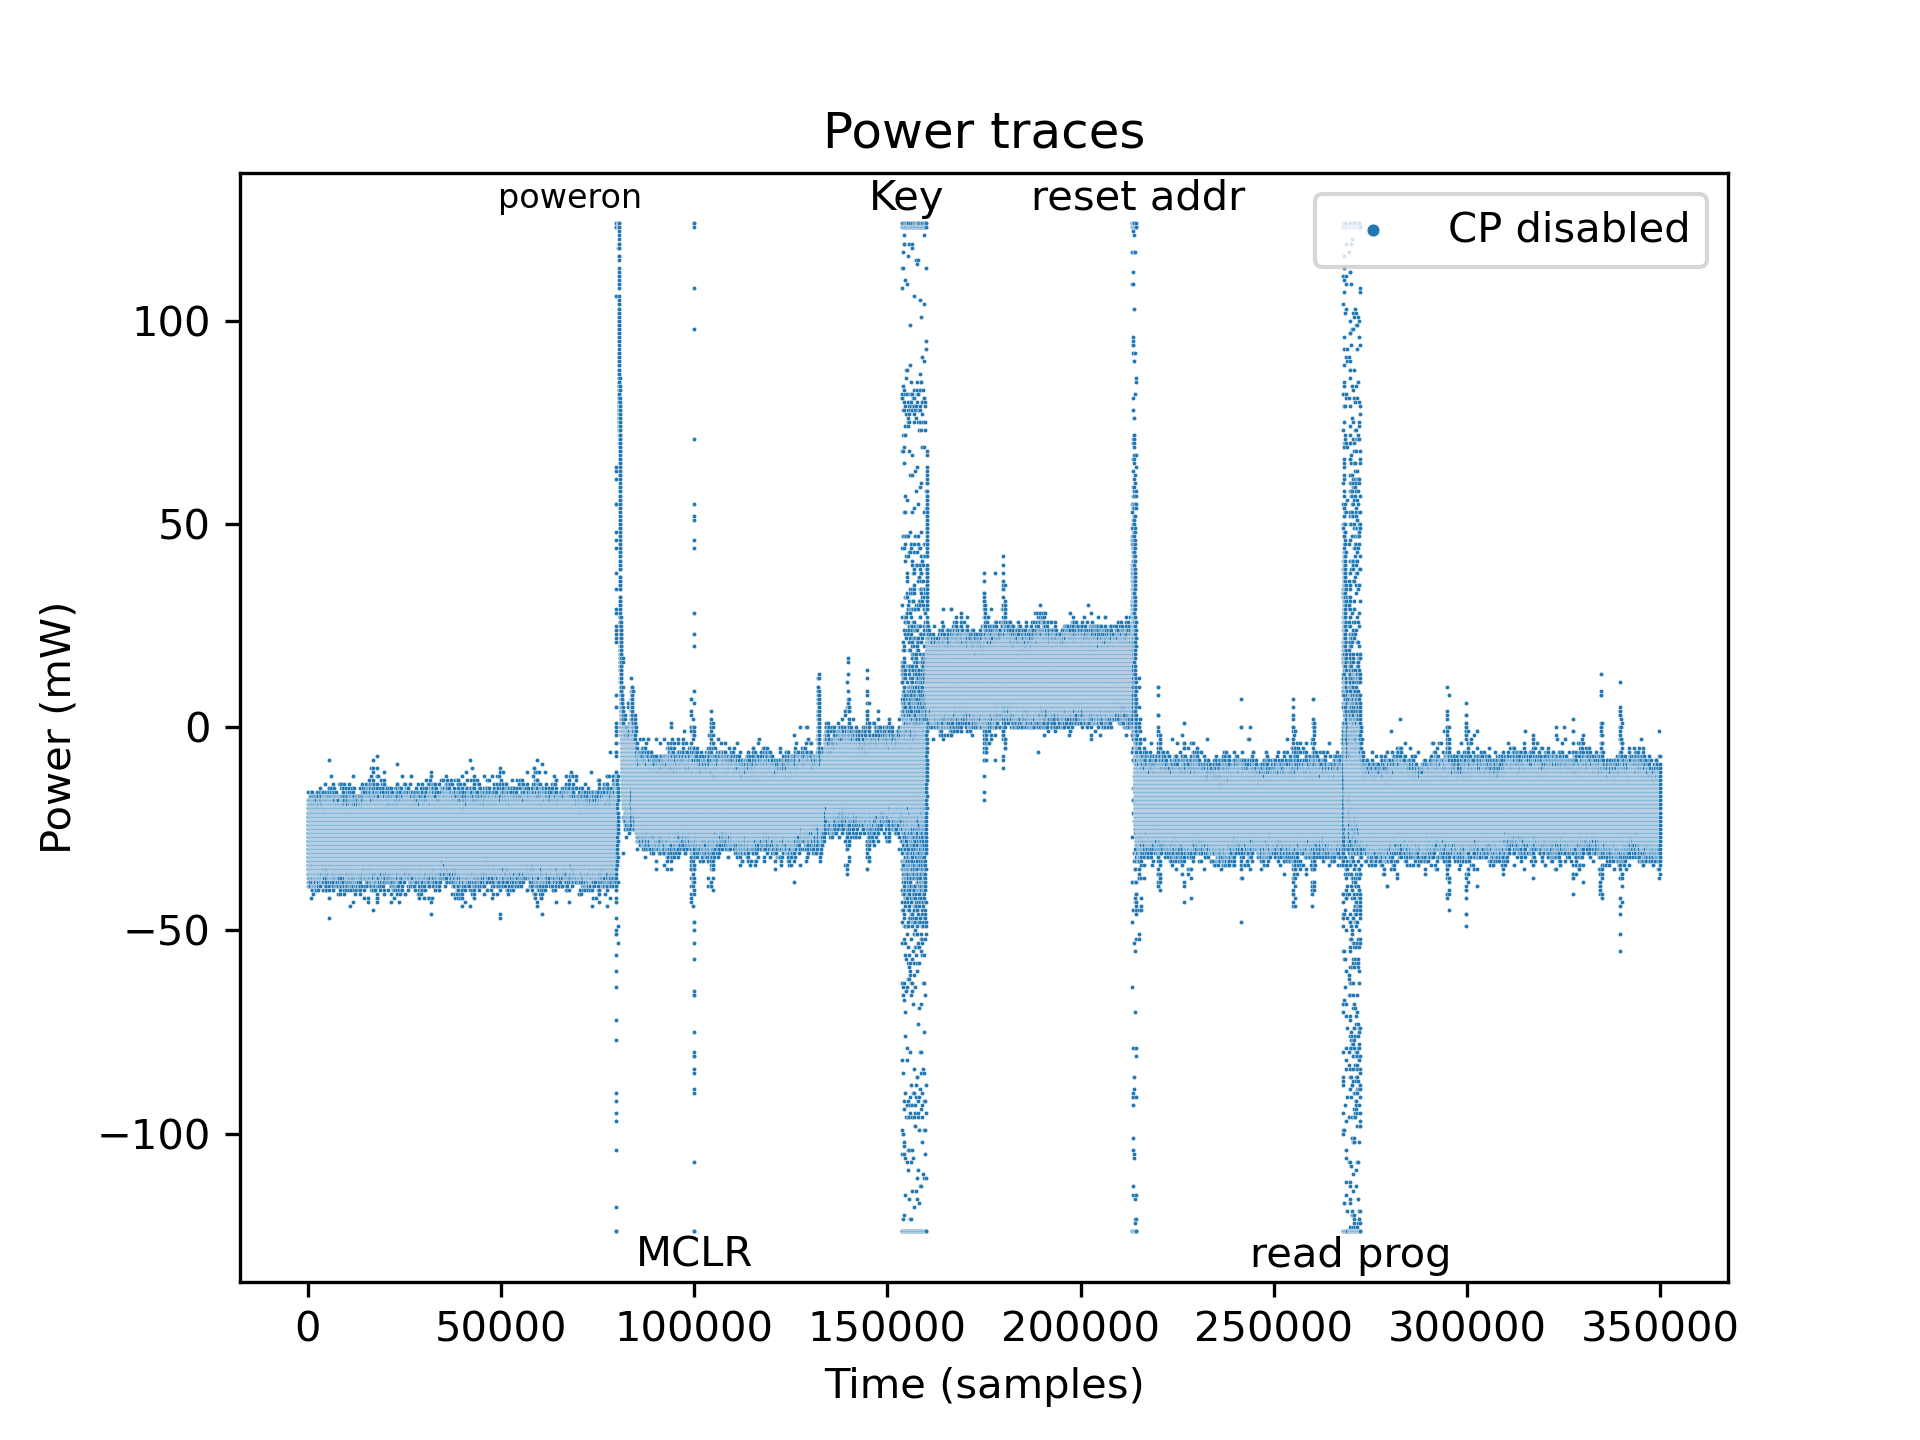
\includegraphics[width=.75\textwidth]{seaborn_power_trace.png}
	\caption{Power trace of a programming session}
	\label{fig:powertrace}
\end{figure}

\subsection{Previous work}
No previous work on this specific device or chip series has been found, but different PICs were targeted in the past.

Other chips of the PIC family implemented code protection differently, for example allowing to set code protection on memory blocks (groups of pages). As it was possible to erase a single block, it was also possible to clear the code protection on that block, and then to program it with new code. This is an attack vector, as it allows to fit a small program in the newly unprotected block that can then dump over the serial port the content of the remaining protected blocks \cite{meriac2010heart}. This approach is not feasible on the PIC16F1936, as the code protection is not implemented on a per-page basis, and write/erase commands at page granularity are ignored when the global code protection is enabled.

Others managed to bypass the code protection shining UV light on the memory cells that store the code protection bit \cite{bunniepic}, thus erasing them ionizing the silicon in the transistor's gate. I have decided not to follow this approach as it is necessary to deal with strong acids to decap the chip. While not impossible per se, I wanted to avoid it if possible.

Someone already attempted, apparently unsuccessfully, to bypass the code protection by means of voltage glitching \cite{silviocopyprotection}. The presentation's slides are not available, and I have not been able to contact the author to ask for more information.



\section{Hardware}
I have decided to build my glitching setup around the MAX4619 \cite{maxim:MAX4617-MAX4619} high speed switch. This chip can be used to switch the power supply of the target between two different sources, and should be fast enough to be used for voltage glitching. It was successfully used by others to attack more modern, capable microcontrollers \cite{gerlinskyLPC}.

The switch is controlled by a Raspberry Pi Pico, which was picked due to its availability and low cost. Also, the PIO subsystem of the Pico allows to generate very precise pulses, which is a requirement for any kind of glitching. This will be discussed in \autoref{sect:software}.

The schematic for the final version of the hardware can be seen in \autoref{app:hardware}.



\section{Software}\label{sect:software}
To keep things simple and minimizing unnecessary complexity, the software component project is made of two main parts that talk over USB serial.

\subsection{Pico firmware}
The firmware running on the Raspberry Pi Pico is written in plain C on top of the \texttt{pico-sdk}\footnote{\url{https://github.com/raspberrypi/pico-sdk}}. This program handles the low level details of both glitching and communicating with the \gls{dut}.

The Pico is an ARM Cortex M0, and as such supports \gls{xip}, with an additional cache to allow executing at the nominal 125 MHz clock speed. The cache introduced timing variability, thus it was necessary to disable it to obtain consistent results; some key functions were moved in RAM.

\subsubsection{PIO}
The IC on the Raspberry Pi Pico board, the RP2040, supports a novel feature called PIO, or Programmable IO. There are 2 PIO blocks, with 4 state machines each, that can be programmed to perform simple tasks, such as generating a pulse of a specific length, or reading a value from a pin and storing it in a register. These state machines run independently of the CPU, and each instruction takes a single clock cycle to execute.

This feature was designed to add support for a variety of peripherals/protocols while maintaining the chip silicon area low. Essentially, it allows to forgo the omnipresent bitbanging of GPIOs to implement custom protocols.

\subsubsection{Glitching}
Glitching requires accurate timing, and the PIO state machines are perfect for this task. A PIO block is used to execute the following algorithm:
\begin{enumerate}
	\item Wait for a specific waveform (rising or falling edge) on the trigger input pin
	\item Count a given number of clock cycles: the glitch delay
	\item Pull the MAX4619 control pin low: \gls{dut} \vdd = glitch tension.\\
		  \textit{Optional: Pull up the trigger output pin high}
	\item Count a given number of clock cycles: the glitch width
	\item Pull the MAX4619 control pin high: \gls{dut} \vdd = nominal tension.\\
		  \textit{Optional: Pull down the trigger output pin}
\end{enumerate}

Once the state machine is configured with the necessary parameters (trigger waveform, delay, width), execution returns to the main program which can continue with its tasks, such as enabling programming mode and issuing commands to the target: the glitch will execute asynchronously.

\subsubsection{ICSP}\label{sect:icsp}
To break the code protection feature of the chip, it is necessary to issue commands to the target in programming mode. While ICSP is a proprietary protocol, many open source implementations exist, but most of them bitbang the GPIOs, taking a lot of CPU time and introducing timing variability.

I have then decided to implement ICSP in PIO assembly code, to minimize the timing variability and to allow the CPU to perform other tasks while the ICSP commands are executed. ICSP functionality is exposed on the same USB serial interface, and the glitch firmware can also be used as a standalone PIC programmer.

\subsection{Controller software}
The controller software is written in Python, and is responsible for orchestrating the glitching process. It accepts options from the command line, and then configures the Pico firmware accordingly communicating over USB serial.

To optimize the glitching process, the search space is explored in random order, and the results are plotted in real time with a QT scatter plot. This allows to monitor the ongoing glitch campaign, and to optimize the parameters as appropriate.

\subsection{ICSP python module}
A small python module is available in \texttt{src/icsp}. It buils upon the firmware feature described in \ref{sect:icsp}, and offers a simple interface to communicate with PIC microcontrollers over ICSP. In the same folder there is also a device library which offers an organized structure, and allows to support other PICs.



\section{Glitching approach}
\subsection{Arithmetic loop}
To validate my setup and verify if the microcontroller could be glitched via voltage glitching, I programmed the target with a simple firmware that would run a loop with arithmetic operations.
%
\begin{flushleft}
	\captionsetup{type=listing}
	\begin{minted}[autogobble]{c}
		IO_RA0_SetHigh();           // Keep output pin high during for loop execution
		for(a = 0; a < 0x10; a++) b--;
		if (a == 0x10 && b == 0) {  // First set either output pin
			IO_RA1_SetHigh();
		} else {
			IO_RA2_SetHigh();
		}
		IO_RA0_SetLow();           // Then finally pull the loop pin down
	\end{minted}
	\caption{Firmware A}
\end{flushleft}
%
This program allowed the glitcher to sync with the \gls{dut} sensing \texttt{PORTA} pin 0, and to easily detect if the glitch was successful or not with \texttt{PORTA} pins 1 and 2.

The above code was indeed glitchable with the following parameters:
\begin{itemize}
	\item \textbf{Power supply}: 3.3V
	\item \textbf{Glitch voltage}: 2.25V
	\item \textbf{Glitch width}: 20 Pico cycles
\end{itemize}

The above parameters were found essentially by trial and error, trying to glitch the target with a wide range of widths and delays, and then adjusting the voltage on the lab power supply. Once I had around 20\% of brownouts, I slightly reduced the glitch width, and then I was able to glitch the \gls{dut} consistently.
Judging by the oscilloscope traces, most of the glitches resulted in the loops being shorter, which means that most likely the glitch was targeting the ALU and resulting in wrong comparisons.

\subsection{Flash readout}
Encouraged by the success of the previous experiment, I tried to glitch program memory (flash) reads. The reasoning behind this is that the code protection bit is stored in a Configuration Word in a special area of the program memory. Since, as mentioned in \autoref{sec:memoryprotection}, the Configuration Word contains value relevant to the chip features during early boot, I assumed that it would be read from flash memory at startup, and possibly stored in registers or flip-flops. Glitching the read operation would then result in the chip booting with a different configuration to the one stored in flash, possibly with code protection disabled.

I then modified the software in the PIC to read out a word from the flash memory, and send it to the glitcher over I2C. In turn, the Pico would forward it to the host software, where it is compared with the expected value. Code in \autoref{lst:flash_readout} populates two global variables with the 14-bit word from memory which will later be sent to the glitcher by the I2C interrupt handler.

The two while loops at the beginning are used to wait for a positive pulse, which is necessary to avoid a potential race condition when the brownout reset of the target is triggered. If the PIC was not waiting for a pulse, on reset it would immediately fetch a value from memory, this time without the glitch, and send it over I2C to the glitcher, which would be still waiting for the value from the previous boot, resulting in a false negative.

\begin{flushleft}
	\captionsetup{type=listing}
	\begin{minted}[autogobble]{c}
		#define FLASH_READ_ADDR 0xAAA
	
		while(!IO_RA1_GetValue()) asm("nop");   // Wait for toggle high...
		while(IO_RA1_GetValue())  asm("nop");   // ...and low
	
		I2C_Open(); // From now on we can return data over i2c
		I2C_SlaveSetWriteIntHandler(ReadIntHandler);
		I2C_SlaveSetAddrIntHandler(AddressIntHandler);
	
		// Configure address to read from
		EEADRL = (FLASH_READ_ADDR & 0x00FF);
		EEADRH = ((FLASH_READ_ADDR & 0xFF00) >> 8);
	
		EECON1bits.CFGS = 0;    // Deselect Configuration space
		EECON1bits.EEPGD = 1;   // Select Program Memory
	
		IO_RA0_SetHigh();       // Keep output pin high during memory read operation
		EECON1bits.RD = 1;      // Initiate Read
		NOP();
		NOP();
		IO_RA0_SetLow();        // Then pull the loop pin down
		datl = EEDATL;
		dath = EEDATH;
	
		while(1) asm("nop");
	\end{minted}
	\caption{Firmware B}\label{lst:flash_readout}
\end{flushleft}

I optimistically expected to be able to glitch the target as easily as before, potentially with minor adjustments to the glitch parameters, but unfortunately this was not the case. I did manage to get wrong data from the program memory, but all the glitches did yield the same unexpected value: \texttt{0x0}, the default initialization value for the global variables.

\begin{center}
	\captionsetup{type=figure}
	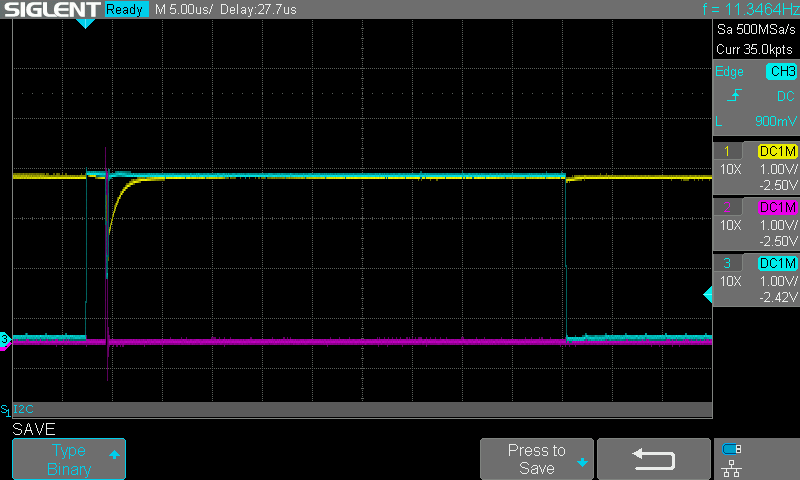
\includegraphics[width=.75\textwidth]{flash_glitches/scope_trace.png}
	\caption{Glitching the flash readout\\Channel 1: SCL \quad Channel 2: Glitch trigger out \quad Channel 3: PIC \texttt{PORTA} pin 0}
	\label{fig:flash_glitch_trace}
\end{center}

As shown in \autoref{fig:flash_glitch_trace}, for the glitch to succeed the delay had to be relatively small, thus the glitch had to be triggered very early in the glitch window. Looking at \autoref{lst:flash_readout}, we notice that the output pin is pulled up just before \texttt{EECON} register's bit \texttt{RD} is set to 1. I speculate that this glitch might be interfering with the register write, effectively not triggering the flash read from the memory subsystem, while the flash peripheral itself operates unaffected.

\subsection{Code protection}
Not succeeding in glitching the flash readout, I decided to analyze the power consumption of the PIC16F1936 during the boot process with and without code protection enabled.

Seeing a difference in the power consumption after a certain amount of time from boot would imply that the code protection bit has been read by that point, and that I could reduce the search space for a suitable glitch. Given that the code protection bit is stored near other values important for the chip configuration, as mentioned in \autoref{sec:memoryprotection}, I expected to see a difference in power consumption at early boot, potentially even before the \mclr pin is brought to \gls{vil}.

The power consumption was measured with an Ohmite APC0805T49R9Z 49,9$\Omega$ precision resistor in series with the ground pin of the PIC, and my Siglent SDS1104X-E oscilloscope. Having this oscilloscope an 8-bit ADC, the measurements are probably not very accurate. Furthermore, the ground pin of the PIC is shared with the ground pin of the Raspberry Pi Pico, thus with my laptop. This setup can't by any means be considered accurate, however it should be good enough to see a difference in power consumption between the two configurations with.

To compare the traces, I borrowed the mathematical tools from \gls{cpa}, namely the Pearson correlation coefficient (\autoref{eq:pearson}) and the \gls{hamweight} of the difference between the two traces. I chose the \gls{hamweight} over \gls{hamdist} because I expected the register or flip-flop to start in an empty state, thus the two leakage models would be equivalent.

\begin{equation}\label{eq:pearson}
	r_{xy} =\frac{\sum ^n _{i=1}(x_i - \bar{x})(y_i - \bar{y})}{\sqrt{\sum ^n _{i=1}(x_i - \bar{x})^2} \sqrt{\sum ^n _{i=1}(y_i - \bar{y})^2}}
\end{equation}

Acquiring 100 traces per configuration, I stored them in the Measurements matrix \(MM\), where each row is a trace, and each column is a sample. I also have the Power-prediction matrix \(PP\), a \((200, 1)\) column matrix with the hamming weight of the Configuration Word 1 with and without code protection.

\[
MM = 
\begin{bmatrix}
	t_{\overline{\footnotesize CP}1}[1] & t_{\overline{\footnotesize CP}1}[2] & \dots & t_{\overline{\footnotesize CP}1}[350000] \\
	\vdots & \vdots & \ddots & \vdots \\
	t_{\overline{\footnotesize CP}100}[1] & t_{\overline{\footnotesize CP}100}[2] & \dots & t_{\overline{\footnotesize CP}100}[350000] \\
	t_{\footnotesize CP1}[1] & t_{\footnotesize CP1}[2] & \dots & t_{\footnotesize CP1}[350000] \\
	\vdots & \vdots & \ddots & \vdots \\
	t_{\footnotesize CP100}[1] & t_{\footnotesize CP100}[2] & \dots & t_{\footnotesize CP100}[350000]
\end{bmatrix}
\qquad \qquad
PP =
\begin{bmatrix}
	\text{HW}(\mbox{\texttt{0x3FFF}}) \\
	\vdots \\
	\text{HW}(\mbox{\texttt{0x3FFF}}) \\
	\text{HW}(\mbox{\texttt{0x3F7F}}) \\
	\vdots \\
	\text{HW}(\mbox{\texttt{0x3F7F}})
\end{bmatrix}
\]

The Pearson correlation coefficient is then calculated over the two matrices by column, and the results are plotted in \autoref{fig:trace_corr} along with a single powertrace to easily identify the boot stages. When the correlation value is close to 1, power consumption in that instant is directly related to the state of the code protection bit. Comparing this picture with \autoref{fig:powertrace}, we notice that there is high correlation in 3 key moments:
\begin{itemize}
	\item The first peak, when the chip is powered on. At this resolution, this is probably due to measurement error, but further analysis could be done focusing on this moment.
	\item After the ICSP key has been sent to the target, and before first ICSP command is issued. I have no explanation for this, but it signals the fact that by this point the chip already knows if code protection is enabled or not.
	\item The last peak is the data readout from program memory. This is expected, as no data will be sent to the programmer if code protection is enabled, thus power consumption will be lower.
\end{itemize}

\begin{figure}[htbp]
	\centering%
	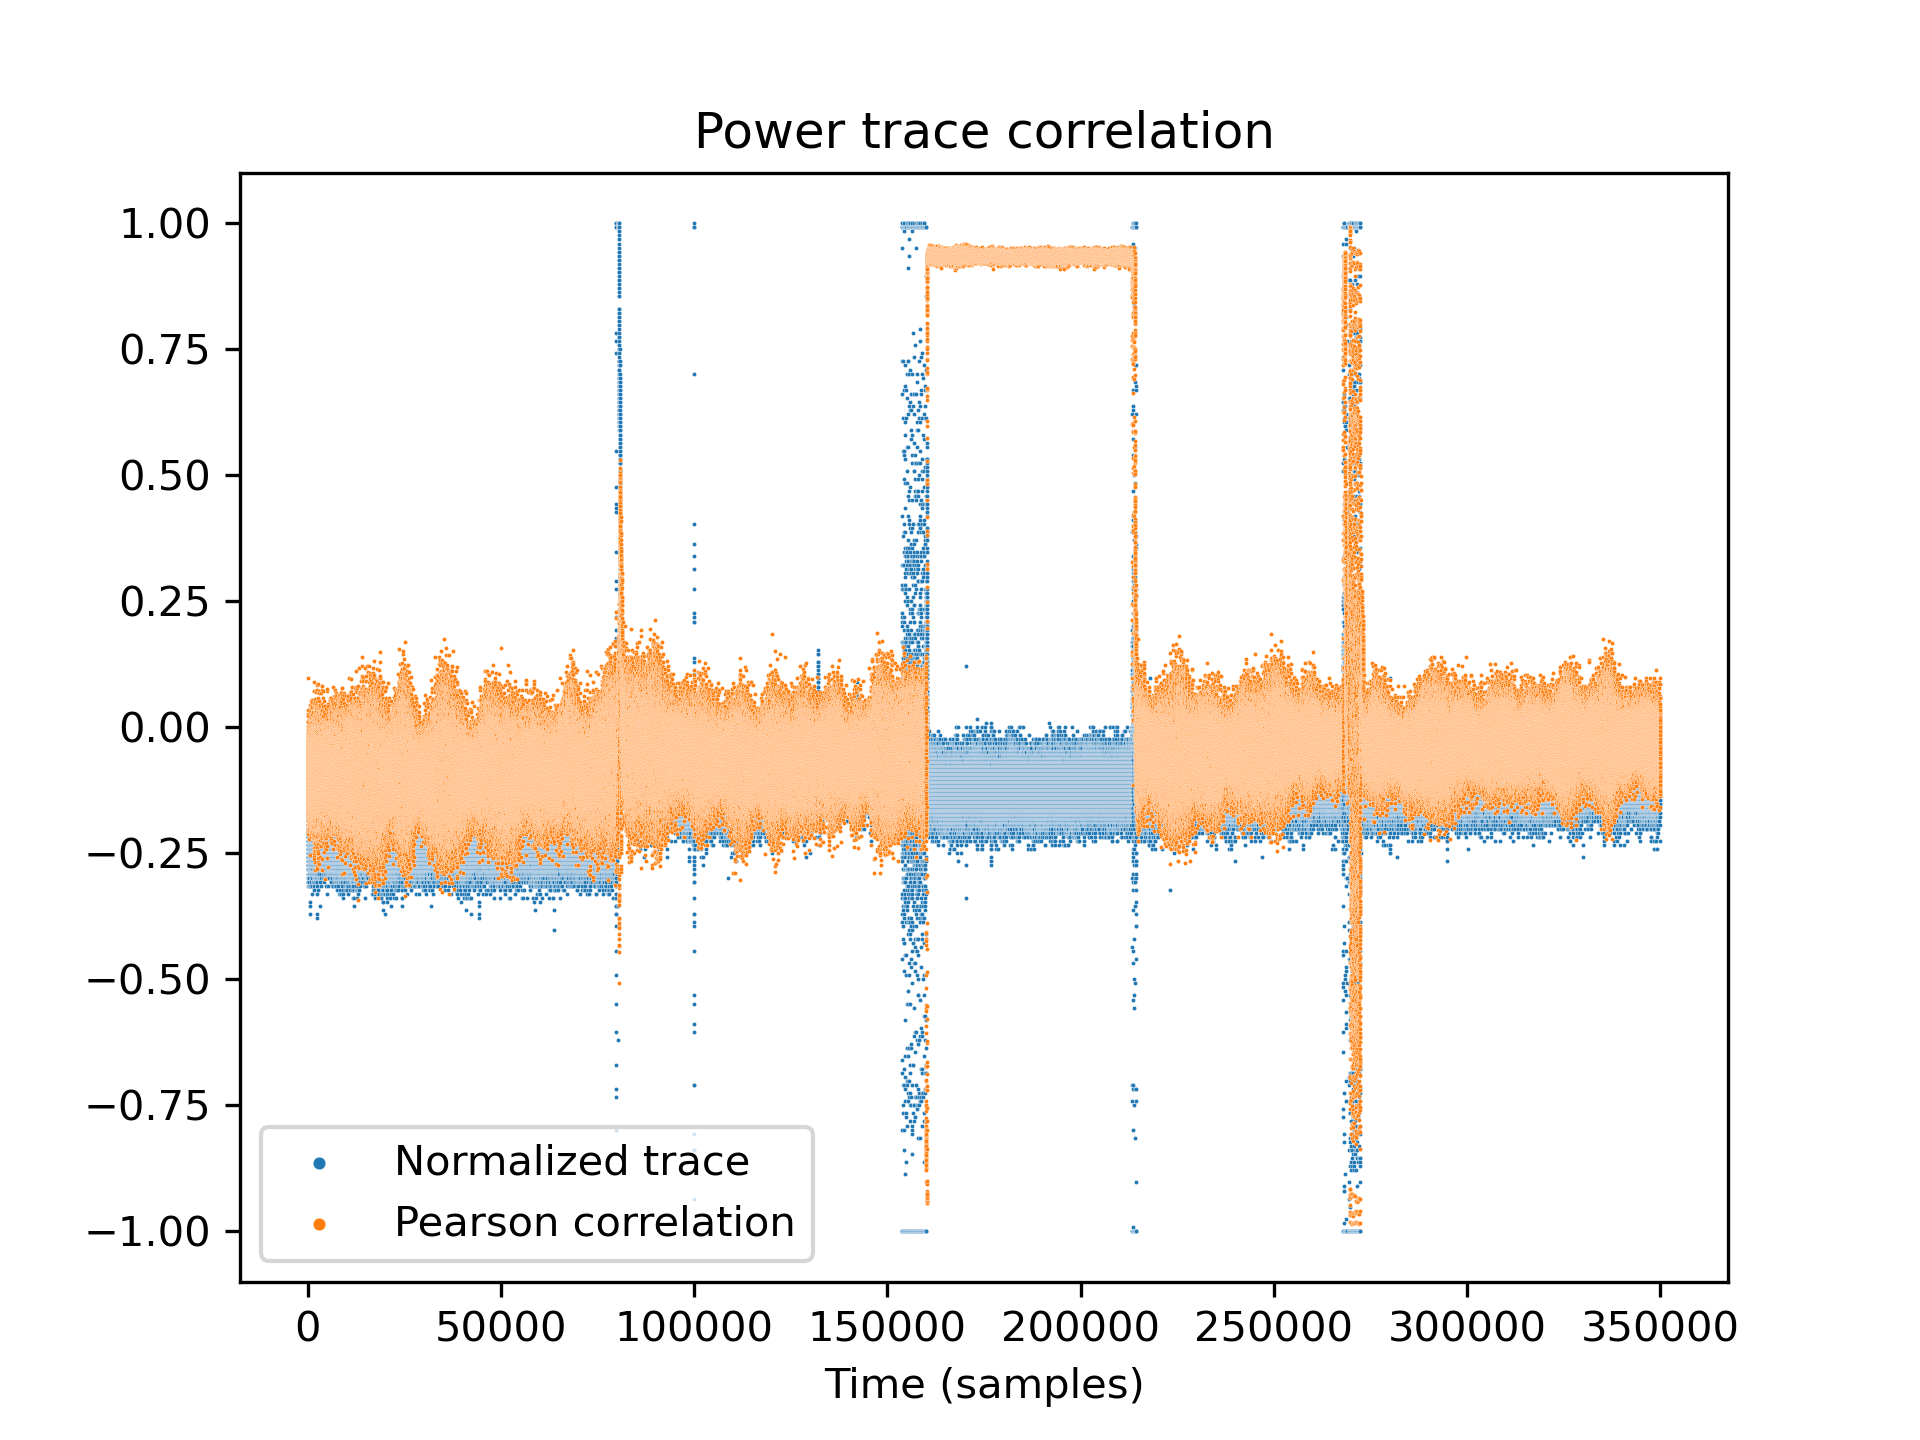
\includegraphics[width=.75\textwidth]{seaborn_trace_correlation.png}
	\caption{Pearson correlation coefficient between the power traces with and without code protection}
	\label{fig:trace_corr}
\end{figure}

The second peak is the most interesting, as it tells us that the check for code protection status is probably done once at boot, and not on a per-read basis. This is promising as, if a glitch is successfully obtained, it will be possible to read the entire memory. Otherwise, it would have been necessary to repeat the glitch for each read.

What is missing in this picture is a clear correlation during early boot, something similar to an if-then branch being executed right after the code protection bit is read, which I had hoped to find to pinpoint the exact moment when the code protection bit is read. This was somewhat expected since, as stated in \autoref{sec:picfeatures}, these devices do not employ a bootloader, and apparently there is no difference in peripheral initialization between the two configurations.

\section{Lessons learned and future work}



\clearpage%
\printglossary[type=\acronymtype]%
\printglossary%
{
\raggedright%
\bibliographystyle{IEEEtran}
\bibliography{bibliography}
}

\clearpage%
\begin{appendix}
\section{Hardware}\label{app:hardware}
\begin{center}
	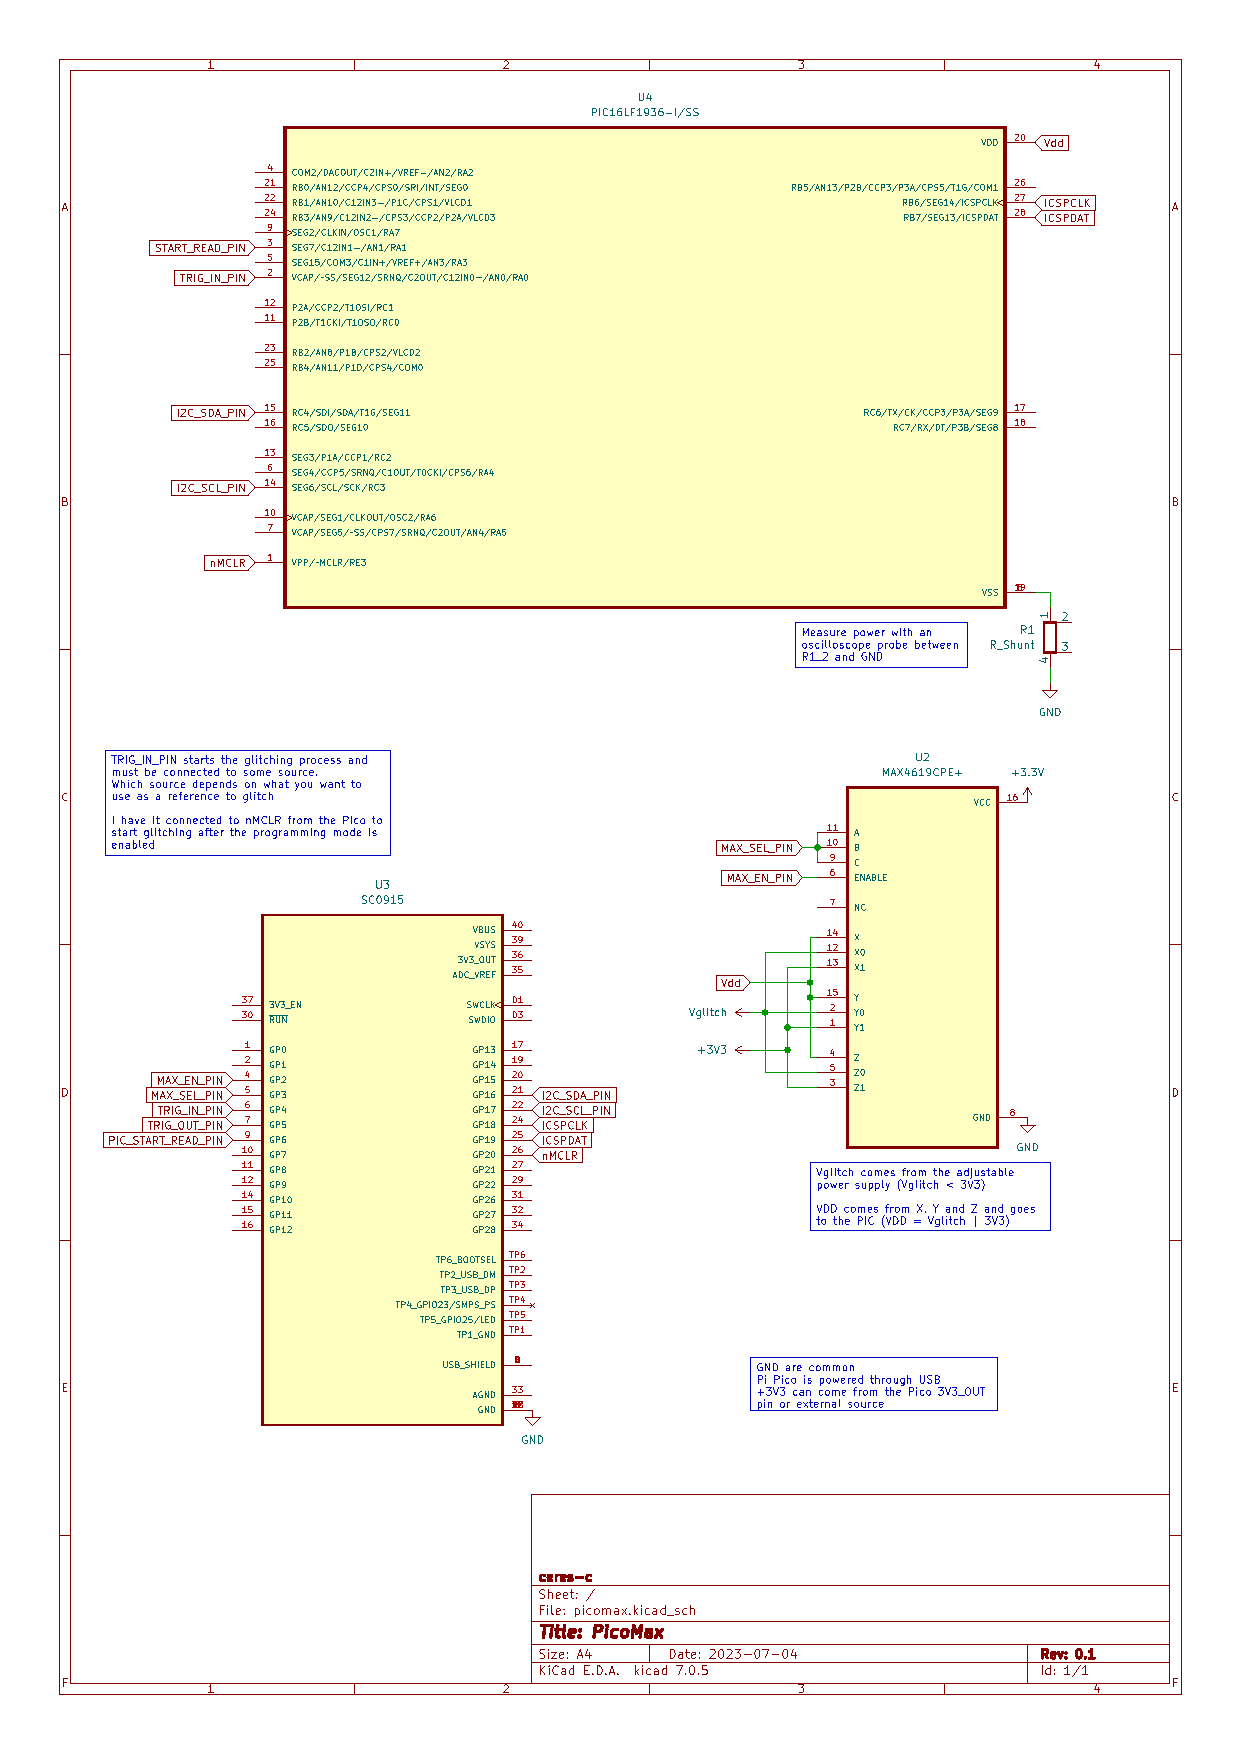
\includegraphics[height=.95\textheight]{../hardware/schematic.pdf}
\end{center}
\end{appendix}

\end{document}
